
\section{Capacity I: Definition and examples}
\label{sec:33}




\subsection{Definition}

\paragraph{A communication system}
A source produces a message $W$, encodes it into a sequence $X^n$ and sends it through a channel.\\
~\\
The receiver obtains a corrupted version $Y^n$ and decodes it to some estimate $\hat{W}$ of $W$.

\begin{center}
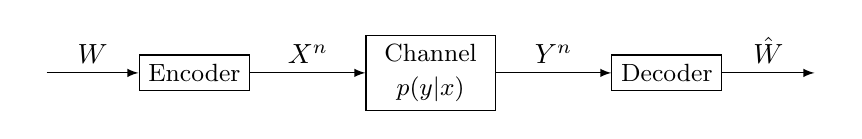
\begin{tikzpicture}[auto]
	\node (s) at (0,0) {}; %{\small{Message}};
	\node[draw] (e) at (2,0) {\small{Encoder}};
	\node[draw, text width=4em, text badly centered] (c) at (5,0) {\small{Channel} \small{$p(y|x)$}};
	\node[draw] (d) at (8,0) {\small{Decoder}};
	\node (r) at (10,0) {}; %{\small{Estimate}};
	
	\draw[-latex] (s) to node {$W$} (e);
	\draw[-latex] (e) to node {$X^n$} (c);
	\draw[-latex] (c) to node {$Y^n$} (d);
	\draw[-latex] (d) to node {$\hat{W}$} (r);
\end{tikzpicture}
\end{center}





\paragraph{Discrete channel}


A \Define{discrete channel} consists of an input alphabet $\alphabet{X}$, and output alphabet $\alphabet{Y}$, and a probability transition matrix $p(y | x)$ that expresses the probability of observing the output symbol $y$ given that we send the symbol $x$.

The channel is called \Define{memoryless} if the probability distribution of the output only depends on the input at that time and is conditionally independent of previous inputs or outputs.

The \Define{channel capacity} of a discrete memoryless channel is defined as
\[
	C = \max_{p(x)} I(X;Y).
\]

Intuitively, the mutual information $I(X.Y)$ is the amount of information the output $Y$ has about the input $X$: that's the amount of information that has been successfully transmitted through the channel. Changing the input distribution $p(x)$ amounts to different sorts of ``encoding'' the data: finding the best input that allows for the most information transmitted through the channel.

The mathematical definition of the capacity makes sense: for a given channel, the output probability distribution $p(y)$ is a function of the input probability distribution $p(x)$:
\[
    p(y) = \sum_x p(x) p(y | x),
\]
and hence the mutual information $I(X;Y)$ is a function of $p(x)$.

\subsection{Examples}

\paragraph{Noiseless binary channel}
Suppose that the channel can carry one bit and it is perfect: $p(y|x) = 1$ if $y=x$. Then $I(X;Y) = H(X)$, which is maximised for $p(x) = (1/2, 1/2)$. 
Thus,
$$
	C = 1.
$$ 



\paragraph{Noisy typewriter}
The alphabet is $\mathbb{Z}_{2q}$ and the input is either unchanged with probability $1/2$ or turned to the next symbol with probability $1/2$:
$$
	p(x|x) = p(x+1 \mod 2q | x) = \frac{1}{2}.
$$

(give figure.)

\begin{theorem}
The \Important{capacity of the noisy typewriter} is $\log q$.
\end{theorem}

\begin{proof}
The proof contains two parts. 

Firstly, we prove that the mutual information is always upper bounded by $\log q$. We have
\begin{align*}
	I(X;Y) &= H(Y) - H(Y|X)\\
	&= H(Y) - 1 \le \log (2q) - 1 = \log q.
\end{align*}

The second part is to exhibit an input distribution that matches our upper bound. Here, we reach capacity if we send every other symbol equiprobably, i.e. 
\[
	p(x) = \begin{cases}
	\frac{1}{q} & \text{if } x \equiv 0 \mod 2\\
	0 & \text{if } x \equiv 1 \mod 2,
	\end{cases}
\]
then we see that $H(X) = \log q$ and $H(Y) = \log(2q)$.
\end{proof}



\paragraph{Binary symmetric channel}

\Important{Binary Symmetric Channel}: $x, y \in \{0,1\}$, 
$$
	p(x|x) = 1-p, \quad p(1- x|x) = p.
$$

(give figure)


(Give figure and intuition behind several data points.)

The capacity $C(p)$ of the BSC has a few intuitive properties.
\begin{enumerate}
    \item $C(0) = 1$: in this case the channel is perfect.
    
    \item $C(p) = C(1-p)$: making that switch amounts to changing the roles of $0$ and $1$ at the destination.
    
    \item $C(1/2) = 0$: in this case, $Y$ receives random noise.
\end{enumerate}

\begin{theorem}
The capacity of a BSC with crossover probability $p$ is
\[
	C(p) = 1 - H(p).
\]
\end{theorem}


\begin{proof}
$$
	I(X;Y) = H(Y) - H(p) \le 1 - H(p),
$$
with equality if and only if $H(Y) = 1$, which is achieved when the input has a uniform distribution. 
\end{proof}



\subsection{The channel coding theorem}



\begin{definition}
The $n$-th extension of the discrete memoryless channel (DMC) is the channel $(\alphabet{X}^n, p(y^n | x^n), \alphabet{Y}^n)$, where
$$
	p(y_k | x^k, y^{k-1}) = p(y_k | x_k), \quad k=1,\ldots,n.
$$
\end{definition}

We shall use the channel without feedback, i.e. $p(x_k | x^{k-1}, y^{k-1}) = p(x_k | x^{k-1})$ hence
$$
	p(y^n | x^n) = \prod_{i=1}^n p(y_i | x_i).
$$





\begin{definition}
An $(M,n)$ \Structure{code} for the channel $(\alphabet{X}, p(y|x), \alphabet{Y})$ consists of the following:
\begin{enumerate}
	\item An index set $\{1,\ldots,M\}$.
	
	\item An encoding function $X^n : \{1,\ldots,M\} \to \alphabet{X}^n$, yielding codewords $X^n(1), \ldots, X^n(M)$. The set of codewords is called the codebook.
	
	\item A decoding function $g: \alphabet{Y}^n \to \{1,\ldots,M\}$.
\end{enumerate}
\end{definition}

The \Structure{rate} of an $(M,n)$ code is
$$
	R := \frac{\log M}{n} \, \text{bits per transmission.}
$$



\begin{definition}
Conditional probability of error 
\begin{align*}
	\lambda_w &:= \mathrm{Pr}\{g(Y^n) \ne w | X^n = X^n(w)\}\\
	&= \sum_{y^n : g(y^n) \ne w} p(y^n | x^n(w))
\end{align*}

\Structure{Maximal probability of error} $\lambda^{(n)}$ for an $(M,n)$ code is 
$$
	\lambda^{(n)} := \max \{\lambda_w : w \in \{1,\ldots,M\} \}.
$$
\end{definition}

We say a rate $R$ is \Structure{achievable} if there exists a sequence of $(2^{nR}, n)$ codes s.t. $\lambda^{(n)} \to 0$.



The channel coding theorem states that the channel capacity is equal to the maximum rate with which we can transmit data reliably (i.e., with negligible probability of error).

\begin{theorem}[The channel coding theorem]
All rates below capacity $C$ are achievable.\\
Specifically, for every rate $R < C$, there exists a sequence of $(2^{nR}, n)$ codes with maximum probability of error $\lambda^{(n)} \to 0$.\\
~\\
Conversely, any sequence of $(2^{nR}, n)$ codes with $\lambda^{(n)} \to 0$ must have $R \le C$.
\end{theorem}









% %\title{Capacity II\\ The channel coding theorem}

% \subsection{The theorem}

% \paragraph

% \begin{definition}
% The $n$-th extension of the discrete memoryless channel (DMC) is the channel $(\alphabet{X}^n, p(y^n | x^n), \alphabet{Y}^n)$, where
% $$
% 	p(y_k | x^k, y^{k-1}) = p(y_k | x_k), \quad k=1,\ldots,n.
% $$
% \end{definition}

% We shall use the channel without feedback, i.e.
% $$
% 	p(y^n | x^n) = \prod_{i=1}^n p(y_i | x_i).
% $$

% 

% \paragraph

% \begin{definition}
% An $(M,n)$ code for the channel $(\alphabet{X}, p(y|x), \alphabet{Y})$ consists of the following:
% \begin{enumerate}
% 	\item An index set $\{1,\ldots,M\}$.
	
% 	\item An encoding function $X^n : \{1,\ldots,M\} \to \alphabet{X}^n$, yielding codewords $X^n(1), \ldots, X^n(M)$. The set of codewords is called the codebook.
	
% 	\item A decoding function $g: \alphabet{Y}^n \to \{1,\ldots,M\}$.
% \end{enumerate}
% \end{definition}

% The rate of an $(M,n)$ code is
% $$
% 	R := \frac{\log M}{n} \, \text{bits per transmission.}
% $$
% 

% \paragraph
% \begin{definition}
% Conditional probability of error 
% \begin{align*}
% 	\lambda_w &:= \mathrm{Pr}\{g(Y^n) \ne w | X^n = X^n(w)\}\\
% 	&= \sum_{y^n : g(y^n) \ne w} p(y^n | x^n(w))
% \end{align*}

% \Structure{Maximal probability of error} $\lambda^{(n)}$ for an $(M,n)$ code is 
% $$
% 	\lambda^{(n)} := \max \{\lambda_w : w \in \{1,\ldots,M\} \}.
% $$
% \end{definition}

% We say a rate $R$ is \Structure{achievable} if there exists a sequence of $(2^{nR}, n)$ codes s.t. $\lambda^{(n)} \to 0$.\\
% ~\\
% Average probability of error $P_e^{(n)} := \frac{1}{M} \sum_w \lambda_w$.


% 


% \paragraph

% \begin{theorem}[The channel coding theorem]
% All rates below capacity $C$ are achievable.\\
% Specifically, for every rate $R < C$, there exists a sequence of $(2^{nR}, n)$ codes with maximum probability of error $\lambda^{(n)} \to 0$.\\
% ~\\
% Conversely, any sequence of $(2^{nR}, n)$ codes with $\lambda^{(n)} \to 0$ must have $R \le C$.
% \end{theorem}

% 






% \subsection{The Asymptotic Equipartition Property (AEP)}

% \paragraph{The Asymptotic Equipartition Property}

% Analogue of the law of large numbers for information theory.\\
% ~\\
% Context: an information source with probability distribution $p(x)$ keeps producing random variables $X_1,\ldots,X_n$ i.i.d with distribution $p(x)$.\\ 
% ~\\
% Claim: For $n$ large, almost all sequences $X_1,\ldots,X_n$ are very similar, and their behaviour is dictated by the entropy.
% 

% \paragraph{The AEP}

% \begin{theorem}[AEP]
% If $X_1,X_2,\ldots$ are i.i.d $\sim p(x)$, then
% $$
% 	- \frac{1}{n} \log p(X_1,\ldots, X_n) \to H(X) \quad \text{in probability.}
% $$
% \end{theorem}

% \begin{proof}
% Since the $X_i$ are i.i.d, so are $\log p(X_i)$. The weak law of large numbers gives
% \begin{align*}
% 	- \frac{1}{n} \log p(X_1,\ldots,X_n) &= - \frac{1}{n} \sum_i \log p(X_i)\\
% 	&\to -\mathrm{E} \log p(X) \quad \text{in probability}\\
% 	&= H(X).
% \end{align*}
% \end{proof}

% 

% \paragraph{Typical sets}

% \begin{definition}
% The \Structure{typical set} $A_\epsilon^{(n)}$ w.r.t. $p(x)$ is the set of sequences $x^n = (x_1,\ldots,x_n) \in \alphabet{X}^n$ such that
% 	$$
% 		H(X) - \epsilon \le -\frac{1}{n} \log p(x^n) \le H(X) + \epsilon.
% 	$$
% \end{definition}

% \begin{theorem}[The AEP for Typical Sequences]
% \begin{enumerate}
% 	\item $\mathrm{Pr}\{A_\epsilon^{(n)}\} \ge 1 - \epsilon$ for $n$ large enough.
	
% 	\item $|A_\epsilon^{(n)}| \le 2^{n(H(X) + \epsilon)}$.
	
% 	\item $|A_\epsilon^{(n)}| \ge (1- \epsilon) 2^{n(H(X) - \epsilon)}$ for $n$ large enough.
% \end{enumerate}
% \end{theorem}

% The typical set has probability nearly $1$, all elements of the typical set are nearly equiprobable, and the number of elements in the typical set is nearly $2^{nH(X)}$.

% 

% %\paragraph{Proof of the AEP}
% %
% %\begin{proof}
% %We've already proved Property 1.\\
% %~\\
% %Property 2:
% %\begin{align*}
% %	1 &= \sum_{x^n \in \alphabet{X}^n} p(x^n)\\
% %	&\ge \sum_{x^n \in A_\epsilon^{(n)}} p(x^n)\\
% %	&\ge \sum_{x^n \in A_\epsilon^{(n)}} 2^{-n(H(X) + \epsilon)}\\
% %	&= 2^{-n(H(X) + \epsilon)} |A_\epsilon^{(n)}|.
% %\end{align*}
% %\end{proof}
% %
% %
% %
% %\paragraph
% %Property 3: let $n$ large enough, then
% %\begin{align*}
% %	1- \epsilon &< \mathrm{Pr}\{A_\epsilon^{(n)}\}\\
% %	&\le \sum_{x^n \in A_\epsilon^{(n)}} 2^{-n(H(X) - \epsilon)}\\
% %	&= 2^{-n(H(X) - \epsilon)} |A_\epsilon^{(n)}|.
% %\end{align*}
% %
% %


% \paragraph{Example of the AEP}
% Consider $n$ coin flips $X_1,\ldots,X_n$, where heads (1) has probability $p$ and tails (0) probability $1-p$.\\
% We expect to see around $np$ heads on average, and all runs with roughly $np$ heads are nearly equiprobable.\\ 
% ~\\
% For any sequence $x^n \in\{0,1\}^n$ with $w$ heads,
% $$
% 	p(x^n)  = p^w (1-p)^{n-w}.
% $$

% The AEP indeed yields
% $$
% 	-\frac{1}{n} \log p(X_1,\ldots,X_n) \to H(p)
% $$
% and more precisely, for typical sets and $n$ large enough:
% \begin{align*}
% 	A_\epsilon^{(n)} &= \{x^n : |w - np| \le \epsilon n/ |\log p - \log (1-p)|\}\\
% 	\mathrm{Pr}\{A_\epsilon^{(n)}\} &\ge 1-\epsilon\\
% 	(1- \epsilon) 2^{n(H(p) - \epsilon)} &\le |A_\epsilon^{(n)}| \le 2^{n(H(p) + \epsilon)}.
% \end{align*}
% 



% %\paragraph{AEP and data compression}
% %???Give this as a practical exercise.
% %
% %Let $X_1,\ldots, X_n$ be i.i.d. We want a short description of this sequence. 
% %
% %\begin{theorem}
% %Let $X^n$ be i.i.d $\sim p(x)$ and $\epsilon > 0$. Then there exists a code which maps sequences $x^n$ of length $n$ into binary strings of length $l(x^n)$ such that the encoding is one-to-one and
% %$$
% %	\mathrm{E} \left[ \frac{1}{n}l(X^n) \right] \le H(X) + \epsilon.
% %$$
% %\end{theorem}
% %
% %Idea of proof:
% %\begin{enumerate}
% %	\item Split $\alphabet{X}^n$ into typical sequences (in $A_\epsilon^{(n)}$) and atypical ones.
% %	
% %	\item In $A_\epsilon^{(n)}$, encode using at most $\log |A_\epsilon^{(n)}| +1 \le n(H(X) + \epsilon) + 1$ bits.
% %	
% %	\item Use brute force enumeration of atypical ones (unimportant: they are unlikely to occur).
% %\end{enumerate}
% %
% %


% \paragraph{The joint AEP}

% \begin{definition}
% $A_\epsilon^{(n)}$: set of jointly typical sequences $(x^n, y^n)$ w.r.t. $p(x,y)$,
% \begin{align*}
% 	A_\epsilon^{(n)} := &\Big\{ (x^n, y^n) \in \alphabet{X}^n \times \alphabet{Y}^n :\\
% 	& \left| -\frac{1}{n} \log p(x^n) - H(X) \right| < \epsilon,\\
% 	& \left| -\frac{1}{n} \log p(y^n) - H(Y) \right| < \epsilon,\\
% 	& \left| -\frac{1}{n} \log p(x^n, y^n) - H(X,Y) \right| < \epsilon \Big\},\\
% \end{align*}
% where
% $$
% 	p(x^n, y^n) = \prod_{i=1}^n p(x_i, y_i).
% $$
% \end{definition}

% 

% \paragraph{The joint AEP}
% \begin{theorem}[Joint AEP]
% Let $(X^n, Y^n)$ be $n$-sequences drawn i.i.d. according to $p(x^n, y^n)$. Then
% \begin{enumerate}
% 	\item $\mathrm{Pr}\{ (X^n, Y^n) \in A_\epsilon^{(n)}\} \to 1$ as $n \to \infty$.
	
% 	\item $|A_\epsilon^{(n)}| \le 2^{nH(X,Y) + \epsilon}$.
	
% 	\item If $(\tilde{X}^n, \tilde{Y}^n) \sim p(x^n) p(y^n)$, then
% 	$$
% 		\mathrm{Pr}\{ (\tilde{X}^n, \tilde{Y}^n) \in A_\epsilon^{(n)} \} \le 2^{-n(I(X;Y) - 3 \epsilon)}.
% 	$$
% 	Also, for $n$ large enough,
% 	$$
% 		\mathrm{Pr}\{ (\tilde{X}^n, \tilde{Y}^n) \in A_\epsilon^{(n)} \} \ge (1 - \epsilon) 2^{-n(I(X;Y) + 3 \epsilon)}.		
% 	$$
	
% \end{enumerate}
% \end{theorem}
% 


% \subsection{Achievability}

% \paragraph{Intuition}
% The channel coding theorem states that the channel capacity is equal to the maximum rate with which we can transmit data reliably (i.e., with negligible probability of error)\\
% ~\\
% Basic idea: for large block lengths, any channel looks like a noisy typewriter and the channel has a subset of inputs that produce essentially disjoint sequences at the output.\\
% ~\\
% For each typical input $n$-sequence there are roughly $2^{nH(Y|X)}$ possible $Y$ sequences, all of them equally likely.\\
% ~\\
% We wish to ensure that two different $X$ sequences produce different $Y$ sequences.\\
% ~\\
% There are roughly $2^{nH(Y)}$ typical $Y$ sequences, hence roughly $2^{nH(Y) - nH(Y|X)} = 2^{nI(X;Y)}$ different sets: code rate of $I(X;Y)$.
% 

% \paragraph
% We first prove that rates $R < C$ are achievable.\\
% ~\\
% Fix $p(x)$. Generate independently $2^{nR}$ codewords according to the distribution
% $$
% 	p(x^n) = \prod_{i=1}^n p(x_i).
% $$
% The codewords are represented as the rows of a matrix
% $$
% 	\alphabet{C} = \begin{pmatrix}
% 	x_1(1) & \ldots  & x_n(1)\\
% 	\vdots & \vdots & \vdots\\
% 	x_1(2^{nR}) & \ldots & x_n(2^{nR})
% 	\end{pmatrix}
% $$
% The probability of generating a particular code $\alphabet{C}$ is 
% $$
% 	\mathrm{Pr}\{\alphabet{C}\} = \prod_{w=1}^{2^{nR}} \prod_{i=1}^n p(x_i(w)).
% $$
% 

% \paragraph
% Consider the following sequence of events:
% \begin{enumerate}
% 	\item A \Structure{random code} $\alphabet{C}$ is generated.
	
% 	\item Sender and receiver know $\alphabet{C}$ and the channel $p(y|x)$.
	
% 	\item A message $W$ is chosen according to a uniform distribution
% 	$$
% 		\mathrm{Pr}\{W = w\} = 2^{-nR}, \quad w=1,\ldots,2^{nR}.
% 	$$
	
% 	\item The $w$-th codeword $X^n(w)$ is sent over the channel.
	
% 	\item The receiver receives $Y^n$ according to
% 	$$
% 		p(y^n | x^n(w)) = \prod_{i=1}^n p(y_i | x_i(w)).
% 	$$
	
% 	\item The receiver guesses which message was sent using \Structure{typical set decoding}: he declares that $\hat{W}$ was sent if 
% 	\begin{itemize}
% 		\item $(X^n(\hat{W}), Y^n)$ is joint typical and
		
% 		\item $(X^n(w), Y^n)$ is not jointly typical for any other $w$.
% 	\end{itemize}
	
% 	\item Decoding error if $\hat{W} \ne W$. Let $E$ be the error event.
% \end{enumerate}

% 

% \paragraph{Analysis of Probability of error}

% Idea: consider the average over all codes.\\
% %
% %We have
% %\begin{align*}
% 	%Pr(\alphabet{E}) &= \sum_{\alphabet{C}} P(\alphabet{C}) P_e^{(n)} (\alphabet{C})\\
% 	%&= \sum_{\alphabet{C}} P(\alphabet{C}) \frac{1}{2^{nR}} \sum_{w=1}^{2^{nR}} \lambda_w(\alphabet{C})\\
% 	%&= \frac{1}{2^{nR}} \sum_{w=1}^{2^{nR}} \sum_{\alphabet{C}} P(\alphabet{C}) \lambda_w(\alphabet{C}).
% %\end{align*}
% ~\\
% By symmetry of the code construction, the average probability of error averaged over all codes does not depend on the particular index that was sent.\\
% ~\\
% So, let us assume $W=1$ was transmitted. We obtain
% \begin{align*}
% 	\mathrm{Pr}\{E\} &= \sum_{\alphabet{C}} P(\alphabet{C}) P_e^{(n)} (\alphabet{C})\\
% 	&= \mathrm{Pr}\{E | W=1\}.
% \end{align*}

% 

% \paragraph
% Denoting the event $E_w := \{(X^n(w), Y^n) \in A_\epsilon^{(n)}\}$, we have
% \begin{align*}
% 	\mathrm{Pr}\{E | W=1\} &= P(E^c_1 \cup E_2 \cup \ldots \cup E_{2^{nR}})\\
% 	&\le P(E_1^c) + \sum_{w=2}^{2^{nR}} P(E_w).
% \end{align*}

% By the joint AEP, $P(E_1^c) \le \epsilon$ for $n$ large enough.\\
% ~\\
% By the code generation, $X^n(1)$ and $X^n(i)$ are independent, so are $Y^n$ and $X^n(w)$, $w \ne 1$. Hence by the joint AEP,
% $$
% 	P(E_w) \le 2^{-n(I(X;Y) - 3 \epsilon)},
% $$
% whence
% $$
% 	\mathrm{Pr}\{E\} \le 2 \epsilon
% $$
% for $R < I(X;Y) - 3 \epsilon$ and $n$ large enough.
% 

% \paragraph
% We finish the proof as such.
% \begin{enumerate}
% 	\item Choose $p(x)$ which achieves capacity: this replaces $I(X;Y)$ with $C$.
	
% 	\item Get rid of average over codebooks. There exists a codebook $\alphabet{C}$ with average error $\le 2 \epsilon$.
	
% 	\item Throw away half the codewords in $\alphabet{C}$ (the ones with highest $\lambda_w$) to obtain $\alphabet{C}^*$.\\
% 	We have $\lambda^{(n)}(\alphabet{C}^*) \le 4 \epsilon$ and the rate of $\alphabet{C}^*$ is $R - \frac{1}{n} \to R$.
% \end{enumerate}
% 



% \subsection{Converse}

% \paragraph{Fano's inequality}
% The decoder wishes to estimate $X$ with distribution $p(x)$. They observe $Y$, related to $X$ by the conditional distribution $p(y|x)$.\\
% ~\\
% From $Y$, they calculate an estimate $g(Y) = \hat{X}$ of $X$.\\
% ~\\
% Let the probability of error be 
% \[
% 	P_e := \mathrm{Pr}\{ \hat{X} \ne X\}.
% \]

% Fano's inequality relates $P_e$ to $H(X|Y)$.

% \begin{theorem}[Fano's inequality]
% \[
% 	H(P_e) + P_e \log(|\alphabet{X}| - 1) \ge H(X|Y).
% \]
% \end{theorem}
% 

% %This can be weakened to
% %\begin{align*}
% %	1 + P_e \log |\alphabet{X}| &\ge H(X|Y)\\
% %	P_e &\ge \frac{H(X|Y) - 1}{\log |\alphabet{X}|}.
% %\end{align*}


% \paragraph{Proof of Fano's inequality}
% Define an error random variable
% \[
% 	E = \begin{cases}
% 	1 & \mbox{if } \hat{X} \ne X\\
% 	0 & \mbox{if } \hat{X} = X.
% 	\end{cases}
% \]

% By the Venn diagram of entropy,
% \[
% 	H(X|Y) = H(E|Y) + H(X|E,Y) - H(E|X,Y).
% \]

% However,
% \begin{align*}
% 	H(E|X,Y) &= 0,\\
% 	H(E|Y) &\le H(E) = H(P_e),\\
% 	H(X|E,Y) &= (1-P_e) H(X|Y,E=0) + P_e H(X|Y,E=1)
% 	\le P_e \log(|\alphabet{X}| - 1).
% \end{align*}

% Thus $H(X|Y) \le H(P_e) + P_e \log(|\alphabet{X}| - 1)$.
% 




% \paragraph{Converse to the coding theorem}

% We will show that if the probability of error tends to zero, then the code rate must be at most $C$.

% \begin{lemma}[Fano's inequality]
% For a DMC with a codebook $\alphabet{C}$ and the input messages uniformly distributed, let $P_e^{(n)} = \mathrm{Pr}\{W \ne g(Y^n)\}$. Then
% $$
% 	H(W | Y^n) \le 1 + P_e^{(n)} n R.
% $$
% \end{lemma}

% We can easily show that using the channel multiple times does not increase the capacity.

% \begin{lemma}
% Let $Y^n$ be the result of passing $X^n$ through a DMC. Then
% $$
% 	I(X^n; Y^n) \le nC.
% $$
% \end{lemma}


% 


% \paragraph{Proof of converse}

% If $\lambda^{(n)} \to 0$, then $P_e^{(n)} \to 0$.\\
% ~\\
% For each $n$, let $W$ be drawn according to a uniform distribution, then $P_e^{(n)} = \mathrm{Pr}\{\hat{W} \ne W\}$ and
% \begin{align*}
% 	nR &= H(W) = H(W|Y^n) + I(W;Y^n)\\
% 	&\le 1 + P_e^{(n)} nR + nC.
% \end{align*}
% Divide by $n$, take the limit:
% $$
% 	R \le C.
% $$

% 

% %\paragraph{Strong converse}
% %We showed that
% %$$
% %	P_e^{(n)} \ge  1- \frac{C}{R} - \frac{1}{nR} \to 1 - \frac{C}{R}.
% %$$
% %Therefore, if the rate is higher than the capacity, the probability of error is bounded away from zero.\\
% %~\\
% %In fact, there is a \Structure{strong converse}: if $R > C$, then $P_e^{(n)} \to 1$ exponentially. The capacity is a clear dividing point!
% %

\subsection{See further}

Sketch of the proof of achievability?



\subsection{Exercises}

\begin{exercise}
Determine the capacity of the following additive channel, where $X \in \{0,1\}$ and $\mathrm{Pr}\{Z = 0\} = \mathrm{Pr}\{Z = a\} = \frac{1}{2}$ for some real number $a > 0$.\\
~\\
\begin{center}
\begin{tikzpicture}
	\node (x) at (0,0) {$X$};
	\node (y) at (4,0) {$Y$};
	\node (z) at (2,2) {$Z$};
	\node[draw, shape=circle] (p) at (2,0) {$+$};
	
	\draw[-latex] (x) -- (p);
	\draw[-latex] (z) -- (p);
	\draw[-latex] (p) -- (y);
\end{tikzpicture}
\end{center}
\end{exercise}

\begin{remark}
We also use the notation 
$$
	Z = \begin{pmatrix}
		0, & a\\
		\frac{1}{2}, & \frac{1}{2}
	\end{pmatrix}.
$$
\end{remark}



\begin{exercise}
The Z-channel with error probability $p$, also called binary asymmetric channel, is a channel where the transition $0 \to 1$ never occurs.

\begin{center}
\begin{tikzpicture}[auto]
	\node (s0) at (0,3) {$0$};
	\node (s1) at (0,0) {$1$};
	\node (d0) at (3,3) {$0$};
	\node (d1) at (3,0) {$1$};
	
	\node (x) at (-1,1.5) {$X$};
	\node (y) at (4,1.5) {$Y$};
	
	\draw[-latex] (s0) -- (d0);
	\draw[-latex] (s1) to node[pos=0.3] {$p$} (d0);
	\draw[-latex] (s1) to node {$1-p$} (d1);
\end{tikzpicture}
\end{center}

What is the capacity of this channel?
\end{exercise}











